%\newpage
%\captionsetup{font={scriptsize,sc,up,singlespacing}}
\begin{figure}[h] % Figure at bottom of the page ([b] argument, could be "t" for top or "h" for here)
	\centering
	%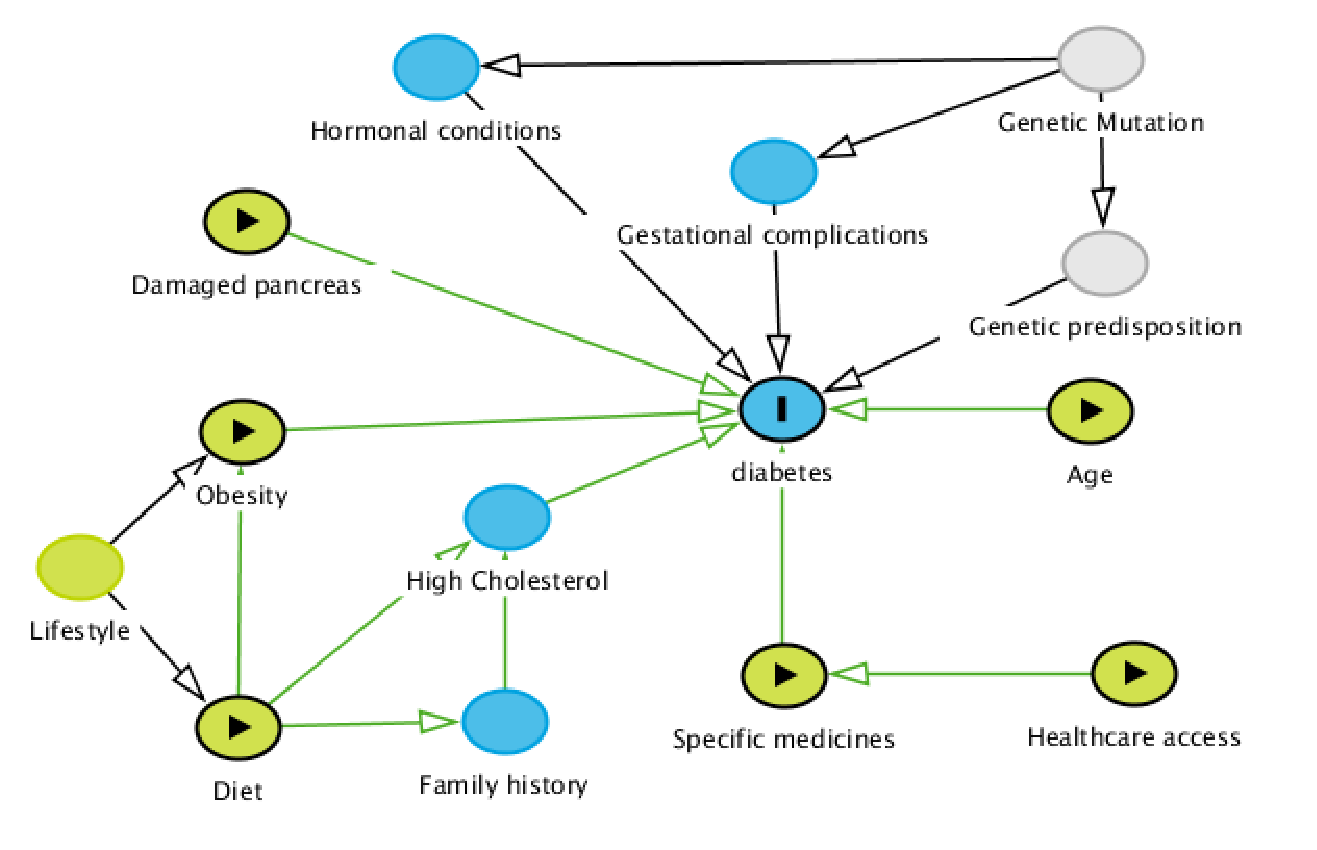
\includegraphics[width=\textwidth]{diabetes-causalmodel.eps}
	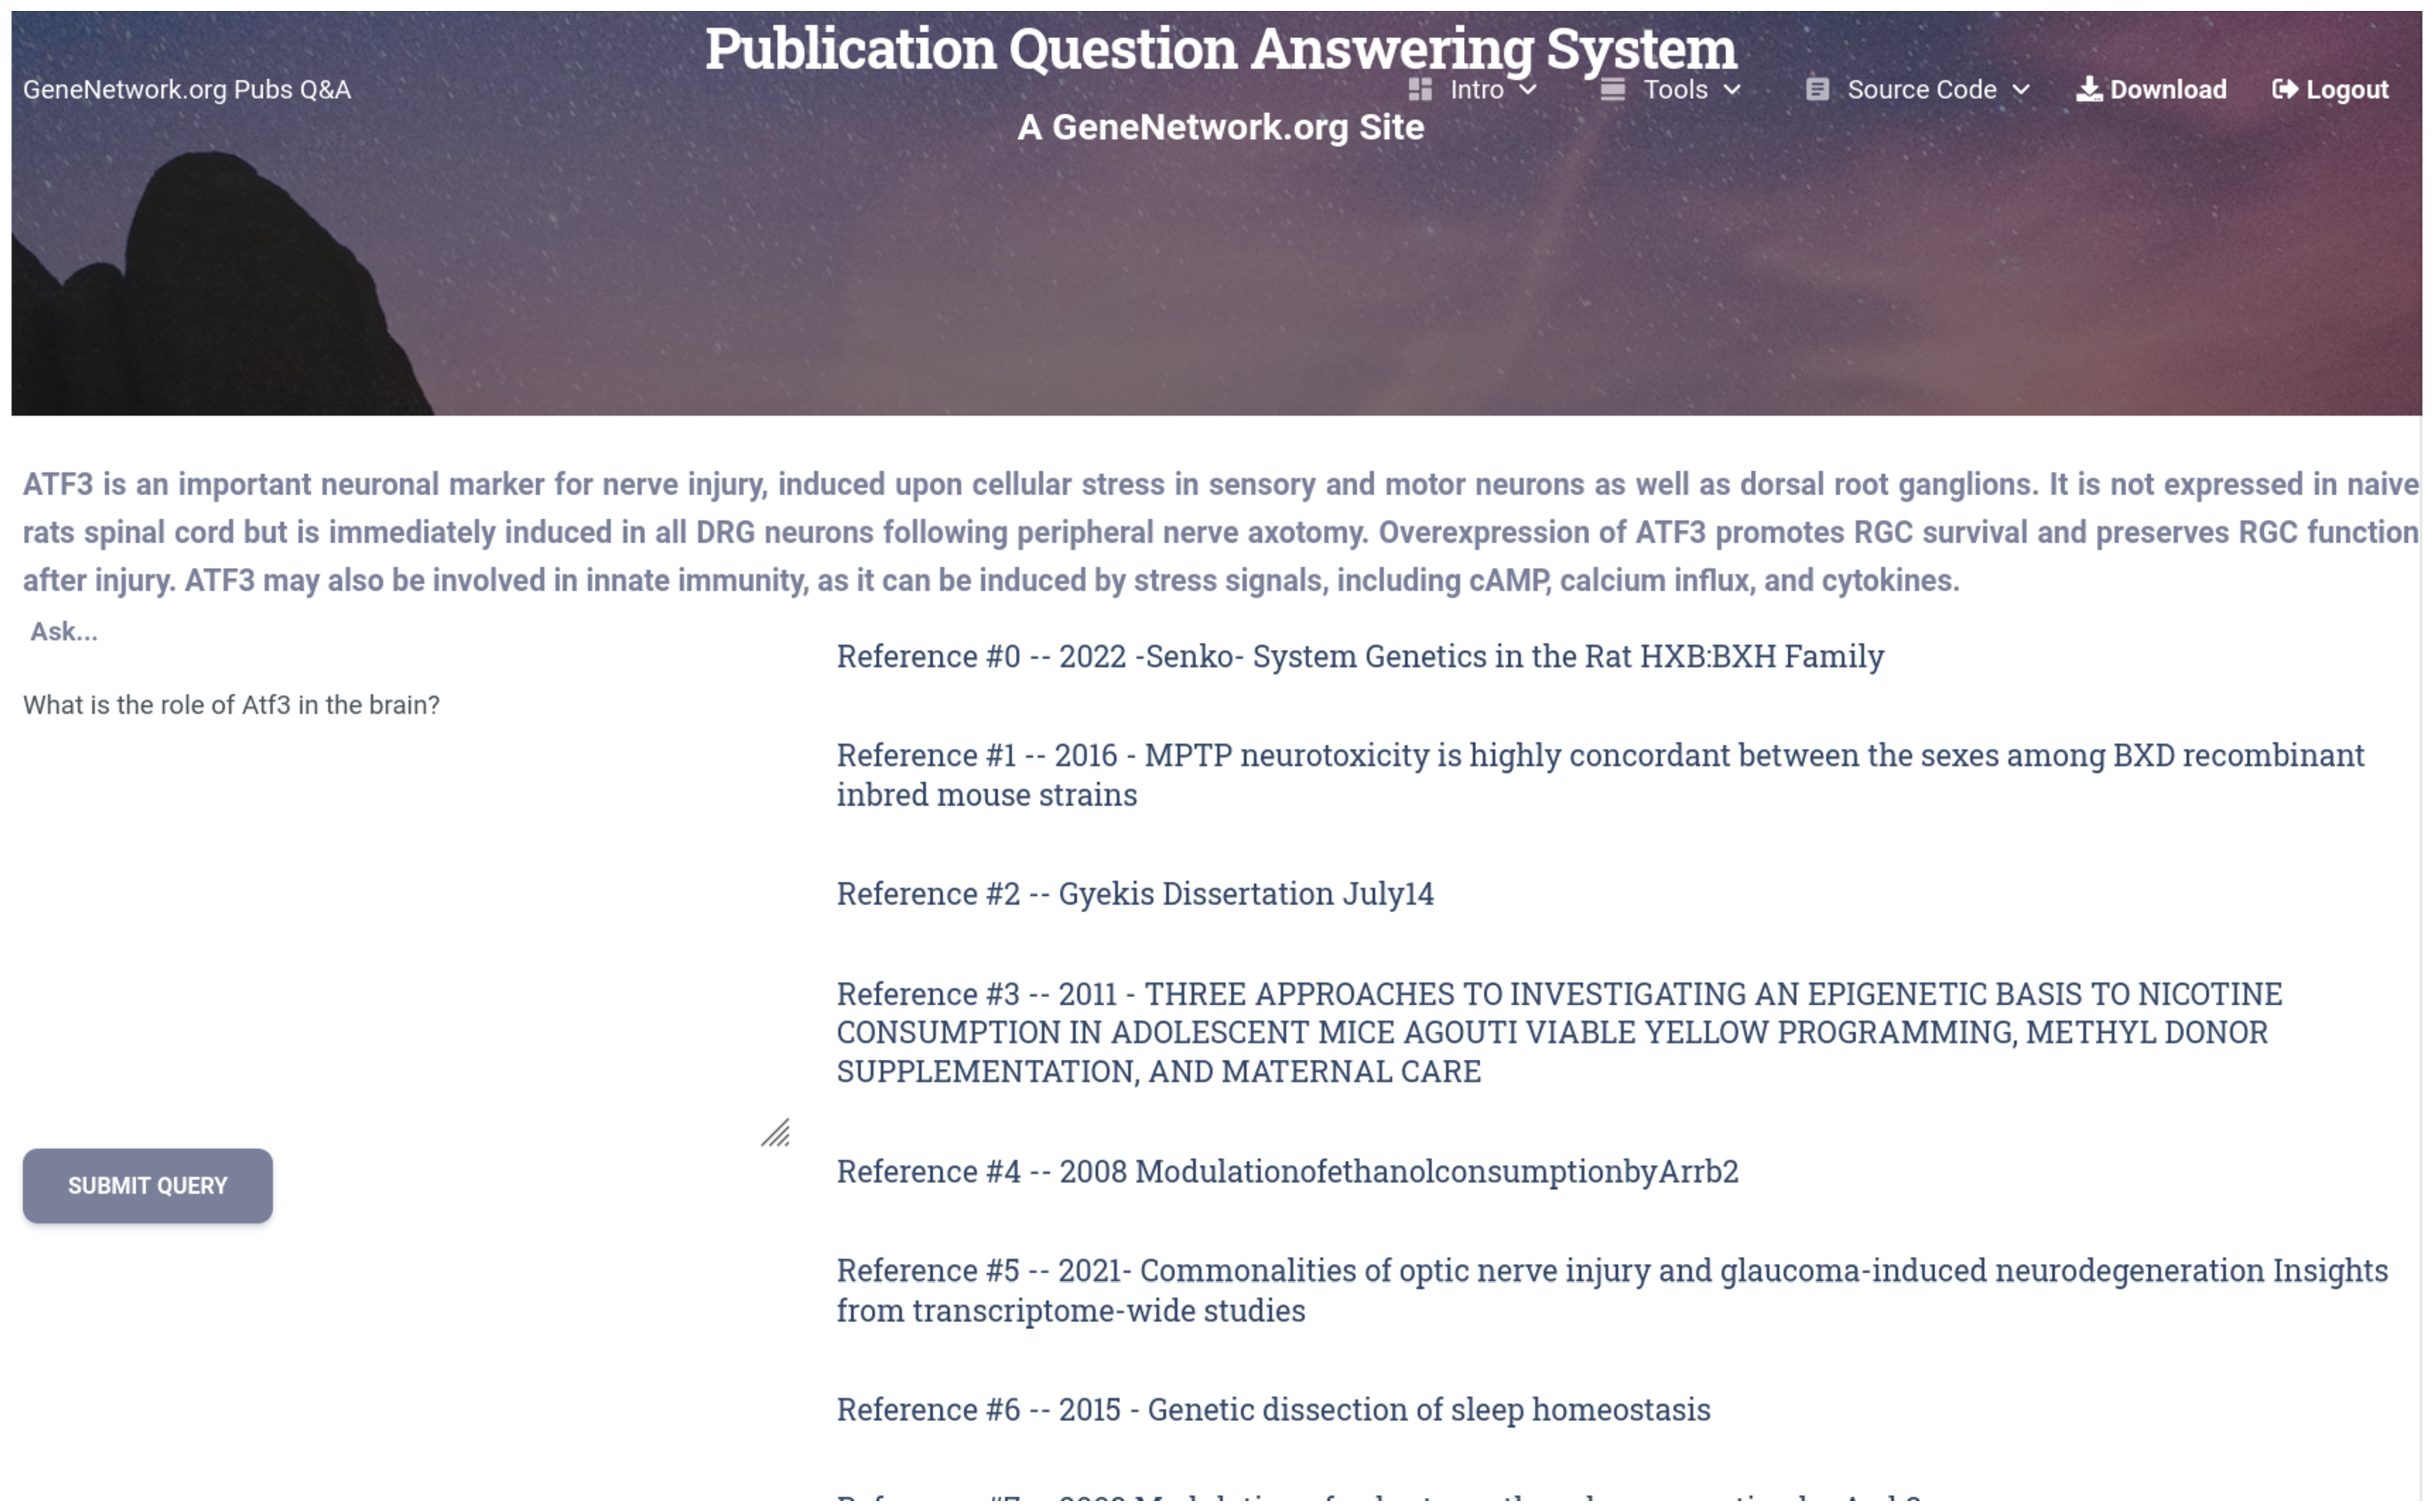
\includegraphics[width=.5\textwidth]{gnqa_atf.eps}
	\caption{ \textbf{GeneNetwork.org Query and Answer Example}
    The same question was asked BingChat and the existing demo of GNQA: `What is the role of Atf3 in the brain?'. 
            }
        \label{fig:gnqa_atf}
\end{figure}
